% ---------------------------------------------------------------------
\subsection{FPGA and the Alveo U50 Board}\label{subsec:fpga}\label{subsec:alveo-u50}
% ---------------------------------------------------------------------
An FPGA (Field-Programmable Gate Array) has programmable logic, made of lookup tables (LUTs) and flip-flops (FFs), and fixed blocks. The DSP block performs multiplications and additions, and the BRAM (Block RAM) is a memory inside the chip \cite{kastner-hls}. This work measures the resources of a circuit by the number of LUTs, FFs, DSPs and BRAMs it uses.

The Alveo U50 is an accelerator card for data centers. Its FPGA, the XCU50, has 872K LUTs, 1,743K FFs, 5,952 DSPs and 1,344 BRAMs of 36~Kb \cite{ds965}. The number of LUTs of the XCU50 is in the middle of the UltraScale+ family \cite{xmp103}.
% FONTE: Kastner et al. 2018, pp. 13-14 e 17.
% FONTE: DS965 v1.8, pp. 1-2 (Tabela 1); XMP103 v1.17, pp. 2-4.
% FONTE (conta): XMP103, 11 dispositivos com menos LUTs que o XCU50, 2 iguais e 8 com mais.

% ---------------------------------------------------------------------
\subsection{High-Level Synthesis}\label{subsec:hls}
% ---------------------------------------------------------------------
High-level synthesis (HLS) starts from a description of the circuit behavior in C or C++ and creates the RTL (Register-Transfer Level) design in Verilog or VHDL. The HLS tool decides which operations run in parallel, where to insert registers to reach the clock frequency, and how to store the data in memory. Logic synthesis then translates the RTL into a netlist of FPGA elements, and placement and routing map each element to a resource of the device \cite{kastner-hls}. Directives (pragmas) guide the HLS decisions, for example the pipelining of loops \cite{ug1399}.
% FONTE: Kastner et al. 2018, pp. 11-13; UG1399, pp. 13-14.

This work also uses loop unrolling and array partitioning. The \texttt{unroll} directive creates several copies of the loop body, which can run in parallel. The copies need to read their data in the same cycle, but a BRAM allows few accesses per cycle. The \texttt{array\_partition} directive divides the array into smaller memories, which the circuit accesses at the same time. The \texttt{cyclic} type distributes the elements among the memories in turn, and the \texttt{complete} type stores each element in FFs \cite{kastner-hls}.
% FONTE: Kastner et al. 2018, p. 41 e pp. 88-90.

% ---------------------------------------------------------------------
\subsection{Static and Dynamic Power}\label{subsec:potencia}
% ---------------------------------------------------------------------
The total on-chip power is the sum of the static power and the design power. The static power comes from the leakage current of the transistors. The design power is the dynamic power, caused by the activity of the circuit. Vivado can estimate the power from the signal activity recorded in a simulation and stored in a SAIF (Switching Activity Interchange Format) file \cite{ug907}.

An average power $P$ held for a time $t$ consumes the energy
\begin{equation}\label{eq:energia}
E = P\, t.
\end{equation}
A circuit with more power can consume less energy per task if it finishes the task in less time.
% FONTE (conta): E = P t.
% FONTE: UG907 v2022.2, pp. 6 e 21.

\subsection{Fixed-Point Representation}\label{subsubsec:ponto-fixo}
The Vitis HLS type \texttt{ap\_fixed}$\langle W, I\rangle$ represents a fixed-point number with $W$ bits in total. The integer part has $I$ bits \cite{kastner-hls}, and the fractional part has $F = W - I$ bits. This work writes the format as $\langle W, I\rangle$.

An overflow occurs when a value does not fit in the integer part. A value that does not fit in the fractional part must be rounded \cite{kastner-hls}. The \texttt{ap\_fixed} type has 7 quantization modes and 5 overflow modes, which gives 35 combinations \cite{ug1399}. Table~\ref{tab:modos-apfixed} describes each mode.

\begin{table}[htbp]
\caption{Quantization and overflow modes of the \texttt{ap\_fixed} type.}
\label{tab:modos-apfixed}
\centering
\footnotesize
\begin{tabular}{p{2.6cm}p{11cm}}
\toprule
\textbf{Mode} & \textbf{Behavior} \\
\midrule
\multicolumn{2}{l}{\textit{Quantization (affects the fractional bits)}} \\
\texttt{AP\_TRN}       & Discards the least significant bits. Rounds toward $-\infty$. \\
\texttt{AP\_TRN\_ZERO} & Rounds toward zero. For positive numbers, it is equal to \texttt{AP\_TRN}. \\
\texttt{AP\_RND}       & Rounds to the nearest value. On a tie, rounds toward $+\infty$. \\
\texttt{AP\_RND\_ZERO} & Rounds to the nearest value. On a tie, rounds toward zero. \\
\texttt{AP\_RND\_MIN\_INF} & Rounds to the nearest value. On a tie, rounds toward $-\infty$. \\
\texttt{AP\_RND\_INF}  & Rounds to the nearest value. On a tie, rounds away from zero. \\
\texttt{AP\_RND\_CONV} & Rounds to the nearest value. On a tie, rounds to the even value. \\
\midrule
\multicolumn{2}{l}{\textit{Overflow (affects the integer bits)}} \\
\texttt{AP\_SAT}       & Saturates at the largest or the smallest representable value. \\
\texttt{AP\_SAT\_ZERO} & Sets the result to zero on overflow. \\
\texttt{AP\_SAT\_SYM}  & Saturates symmetrically: the positive and negative limits have the same magnitude. \\
\texttt{AP\_WRAP}      & Discards the most significant bits that do not fit (two's complement wraparound). \\
\texttt{AP\_WRAP\_SM}  & Discards the same bits, but in sign-magnitude. \\
\bottomrule
\end{tabular}
\legend{Source: \citesp{ug1399}.}
\end{table}
% FONTE: UG1399, pp. 994-995 e 1039-1044.
% FONTE: Kastner et al. 2018, pp. 70-71 (estouro e arredondamento), pp. 73-74 (ap_fixed<W, I>).

\subsection{Latency, Interval and Throughput}\label{subsubsec:latencia-intervalo}
In HLS, a task is a function call. The task latency is the time from the start to the end of a task. The task interval is the time from the start of one task to the start of the next one. A pipelined circuit can start a new task before the previous one ends, so the interval can be smaller than the latency. Many tools call the interval throughput. A larger interval means fewer tasks per unit of time, that is, a lower throughput. The initiation interval (II) is the interval between two data items that enter the pipeline.

In a sequence of tasks, the first task ends after the latency $L$, and each of the next tasks ends one interval $I$ after the previous one \cite{kastner-hls}. So, $n$ tasks end at
\begin{equation}\label{eq:fim-tarefas}
t_n = L + (n-1)\, I.
\end{equation}
\textcolor{blue}{A task in this work is one matrix inversion, and the throughput is measured by the interval between inversions.}
% FONTE: Kastner et al. 2018, pp. 20-22 (Fig. 1.7) e p. 45.

\subsection{Task Pipeline}\label{subsubsec:pipeline-tarefas}
A task can have several steps. \textcolor{blue}{The steps of a task pipeline work at the same time, each one on different data.} So, the next task starts when the previous one finishes the first step. The interval of the whole pipeline is never smaller than the interval of the slowest step \cite{kastner-hls}. \textcolor{blue}{The \texttt{dataflow} directive in HLS creates this pipeline and lets functions and loops overlap \cite{ug1399}.}
% FONTE: UG1399, pp. 787-788 (DATAFLOW) e 855-856 (UNROLL).
% FONTE: Kastner et al. 2018, pp. 113-115.

\subsection{Systolic Array}\label{subsubsec:arranjo-sistolico}
A systolic array is a set of identical processing elements (PEs), in which each PE exchanges data only with its neighbors. Unrolling an inner loop can create this kind of design, with each copy of the loop body as one PE \cite{kastner-hls}.
% FONTE: Kastner et al. 2018, pp. 153 e 180, glossário.

Figure~\ref{fig:sistolico-classico} shows a grid systolic array that computes the Gram matrix of $\mathbf H$. This matrix is Hermitian, so the array computes only the lower triangle. The array reads one row of $\mathbf H$ per cycle. The data enter from the top and from the left and move to the PE below and to the PE on the right. Each PE multiplies its two inputs and accumulates the product. After all rows are read, each PE holds one element of the matrix \cite{wang2021tlbdinsa}.
% FONTE: wang2021tlbdinsa p. 2979, Fig. 14.

\begin{figure}[!ht]
\caption[Lower triangular systolic array that computes a Gram matrix.]{Lower triangular systolic array that computes a Gram matrix. $a_j$ and $b_i$: elements of one row of $\mathbf H$.}
\label{fig:sistolico-classico}
\vspace{4pt}
\centering
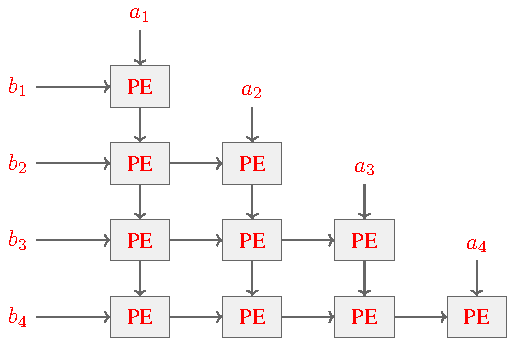
\includegraphics{Images/FLUXO/inversao_cholesky.pdf}
\vspace{4pt}
\legend{Source: adapted from \citesp{wang2021tlbdinsa}.}
\end{figure}
